\begin{tikzpicture}[]

  \tikzstyle{netstyle} = [matrix of nodes,nodes={draw,rectangle,inner sep=0, minimum size=1.5cm},column sep=0cm,row sep=0cm]
  \tikzstyle{cl} = [draw=none,fill=none]
  \tikzstyle{zentral} = [fill=red!70!pagecolor]

  \matrix[netstyle] (mat)
  {
    $(\mat{F})_{1,1}$ & $(\mat{F})_{1,2}$ & $(\mat{F})_{1,3}$\\
    $(\mat{F})_{2,1}$ & |[zentral]| $(\mat{F})_C$ & $(\mat{F})_{2,3}$\\
    $(\mat{F})_{3,1}$ & $(\mat{F})_{3,2}$ & $(\mat{F})_{3,3}$\\
  };


  \draw[<->, thick,transform canvas={xshift=-3mm}] (mat-3-1.south west) -- (mat-1-1.north west) node [midway,sloped,above] {$f$};
  \draw[<->, thick,transform canvas={yshift=-3mm}] (mat-3-1.south west) -- (mat-3-3.south east) node [midway,sloped,below] {$f$};
\end{tikzpicture}

\begin{tikzpicture}[every node/.style={minimum size=1cm},on grid]

  % left front
  \begin{scope}[every node/.append style={yslant=-0.5},yslant=-0.5]
    \shade[right color=gray!10, left color=black!50] (0,0) rectangle +(3,3);
    \node at (0.5,2.5) {$(\mat{F})_{1,1,1}$};
    \node at (1.5,2.5) {7};
    \node at (2.5,2.5) {1};
    \node at (0.5,1.5) {2};
    \node at (1.5,1.5) {4};
    \node at (2.5,1.5) {8};
    \node at (0.5,0.5) {5};
    \node at (1.5,0.5) {3};
    \node at (2.5,0.5) {6};
    \draw (0,0) grid (3,3);
  \end{scope}

  % right front
  \begin{scope}[every node/.append style={yslant=0.5},yslant=0.5]
    \shade[right color=gray!70,left color=gray!10] (3,-3) rectangle +(3,3);
    \node at (3.5,-0.5) {3};
    \node at (4.5,-0.5) {we};
    \node at (5.5,-0.5) {7};
    \node at (3.5,-1.5) {6};
    \node at (4.5,-1.5) {1};
    \node at (5.5,-1.5) {5};
    \node at (3.5,-2.5) {8};
    \node at (4.5,-2.5) {2};
    \node at (5.5,-2.5) {4};
    \draw (3,-3) grid (6,0);
  \end{scope}

  % top
  \begin{scope}[every node/.append style={
      yslant=0.5,xslant=-1},yslant=0.5,xslant=-1
    ]
    \shade[bottom color=gray!10, top color=black!80] (6,3) rectangle +(-3,-3);
    \node at (3.5,2.5) {1};
    \node at (3.5,1.5) {4};


    \node at (3.5,0.5) {7};
    \node at (4.5,2.5) {5};
    \node at (4.5,1.5) {6};
    \node at (4.5,0.5) {8};
    \node at (5.5,2.5) {2};
    \node at (5.5,1.5) {3};
    \node at (5.5,0.5) {he};
    \draw (3,0) grid (6,3);
  \end{scope}
\end{tikzpicture}


\tdplotsetmaincoords{70}{120}
\begin{tikzpicture}[tdplot_main_coords]
  \def\BigSide{5}
  \def\SmallSide{1.5}
  \pgfmathsetmacro{\CalcSide}{\BigSide-\SmallSide}

  % The vertex at V
  \tdplotsetcoord{P}{sqrt(3)*\BigSide}{55}{45}

  \coordinate (sxl) at (\BigSide,\CalcSide,\BigSide);
  \coordinate (syl) at (\CalcSide,\CalcSide,\BigSide);
  \coordinate (szl) at (\CalcSide,\BigSide,\BigSide);

  \draw[dashed]
  (0,0,0) -- (Px)
  (0,0,0) -- (Py)
  (0,0,0) -- (Pz);
  \draw[->]
  (Px) -- ++ (1,0,0) node[anchor=north east]{$x$};
  \draw[->]
  (Py) -- ++(0,1,0) node[anchor=north west]{$y$};
  \draw[->]
  (Pz) -- ++(0,0,1) node[anchor=south]{$z$};

  \draw[thick]
  (Pxz) -- (P) -- (Pxy) -- (Px) -- (Pxz) -- (Pz) -- (Pyz) -- (P);
  \draw[thick]
  (Pyz) -- (Py) -- (Pxy);

  \fill[pattern=north west lines,opacity=0.3]
  (\BigSide,\CalcSide,\CalcSide) -- (\CalcSide,\CalcSide,\CalcSide) -- (\CalcSide,\BigSide,\CalcSide) -- (\BigSide,\BigSide,\CalcSide) -- cycle;
  \draw[dashed]
  (\BigSide,\CalcSide,\CalcSide) -- (\CalcSide,\CalcSide,\CalcSide) coordinate (C) -- (\CalcSide,\BigSide,\CalcSide);

  \fill[pattern=north east lines,opacity=0.3]
  (\BigSide,\CalcSide,\CalcSide) -- (\CalcSide,\CalcSide,\CalcSide) -- (\CalcSide,\CalcSide,\BigSide) -- (\BigSide,\CalcSide,\BigSide) -- (\BigSide,\CalcSide,\CalcSide) -- cycle;
  \draw[dashed]
  (\CalcSide,\CalcSide,\CalcSide) -- (\CalcSide,\CalcSide,\BigSide);

  \draw[thick]
  (szl) -- (syl) -- (sxl) -- (\BigSide,\CalcSide,\CalcSide) -- (\BigSide,\BigSide,\CalcSide) -- (\CalcSide,\BigSide,\CalcSide) -- cycle;

  \node[label=above:$V$,fill,circle,inner sep=1.75pt] at (P) {};
  \node[shift={(-0.5pt,0,0)}] at (C) {$C$};
\end{tikzpicture}

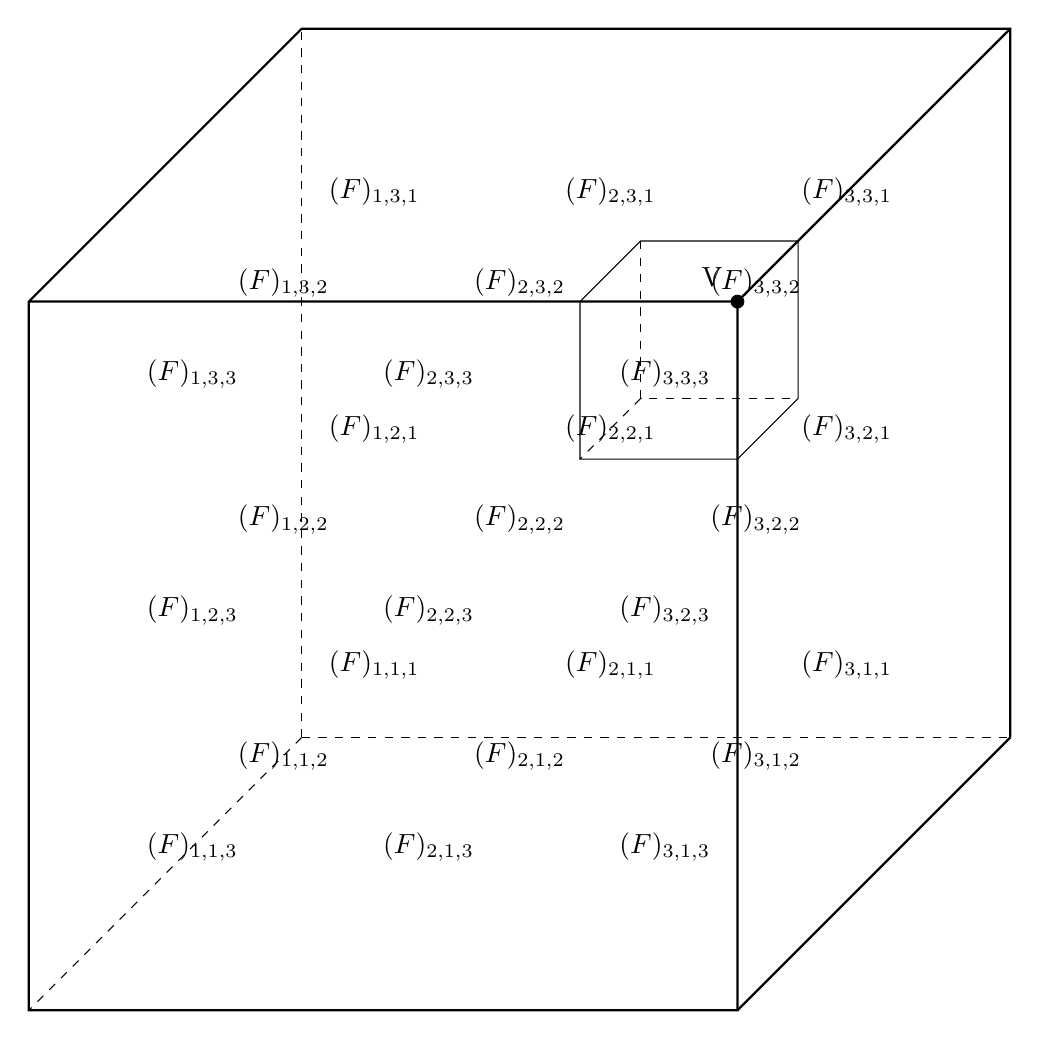
\begin{tikzpicture}
  \draw[thick] (9,0,0) coordinate (x) |- (0,9,0) coordinate [midway] (h) coordinate (y) -- (0,9,9) coordinate (a) -- (0,0,9) coordinate (z) -- (9,0,9) edge (x) -- (9,9,9) coordinate (v) edge (h)
  -- (a);
  \draw [dashed] (0,0,0) coordinate (o) edge (x) edge (y) -- (z);
  \node [circle, minimum size=5pt, inner sep=0pt, fill, label=135:V] at (v) {};
  \draw (v) -- ++(0,0,-2) coordinate (d) -- ++(-2,0,0) coordinate (e) -- ++(0,0,2) |- ++(2,-2,0) coordinate [midway] (f) -- ++(0,0,-2) coordinate (g) -- (d);
  \draw [dashed] (e) -- ++(0,-2,0) coordinate (c) edge (f) -- (g);

  \foreach \x/\xt in {1.5/1,4.5/2,7.5/3} {
    \foreach \y/\yt in {1.5/1,4.5/2,7.5/3} {
      \foreach \z/\zt in {1.5/1,4.5/2,7.5/3} {
        \coordinate (pos) at (\x,\y,\z);
        \node [] at (pos) {$(\ten{F})_{\xt,\yt,\zt}$};
      }
    }
  }

\end{tikzpicture}

%%% Local Variables:
%%% mode: latex
%%% TeX-master: "../figs"
%%% End:
